Wolfenstein 3D was released in May 1992 and created the First Person Shooter genre. The beautiful graphics, high framerate, crisp sounds effect and engaging musics were universally acclaimed. Within a year more than 100,000 units had been sold, bringing fame and a little bit of fortune to the team of people who built it: id Software.\\
\\
The many fans did not stop at beating the game. Because they wanted to modify it and make their own characters and maps, they started to explore and reverse engineer the engine. Within a few months the assets formats were well known and people released mods\footnote{MODified version.} with altered graphics, sounds effects, music and maps. The core of the game however, the 3D engine and the secrets of its speed remained mostly unknown.\\
\\
It was kept secret for an obvious reason: A good game engine was considered the main asset of a game company. As a mean to outperform competitors it was a good business practice to keep other programmers  uneducated in order to gain technological advantage and generate profit.\\
\\
But a few people within id Software did not see things that way. Instead of going along with what was common sense, they wanted to embrace players enthusiasm and fully open the source code to the public. After many internal debate, id Software did the unthinkable: On July 21, 1995 they uploaded a zip archive on \emph{ftp.idsoftware.com} containing the full source code of the engine with all instructions to build it\footnote{They were not totally crazy: They had built a game engine making Wolfenstein 3D obsolete: Doom was released on December 10, 1993}.\\

 \begin{fancyquotes}
   Programming is not a zero-sum game. Teaching something to a fellow programmer doesn't take it away from you. I'm happy to share what I can, because I'm in it for the love of programming.\\
   \\
\textbf{John Carmack - Programmer}
 \end{fancyquotes}\\
\\
Sharing their knowledge was the Right Thing To Do\footnote{The Right Thing To Do was first brought to fame and extensively discussed in "Hackers: Heroes of the Computer Revolution" by Steven Levy". It was also often mentioned in John Carmack journal using the finger protocol.}: It enabled innumerable programers to become better. It had two annex unforeseen consequences:\\
\\
It allowed the software to live long after the target hardware and operating system died. With access to the source, programmers were able to update and port the engine to new hardware and operating systems: Twenty years after the release of Wolfenstein 3D you can still play the game on anything with a CPU, RAM and a framebuffer. \\
\\
A second unexpected side effect was the creation of a window back in time looking right into 1992. As a technical writer on \emph{fabiensanglard.net} I thought i would never take a look at this old thing. But when out of curiosity I took a peek, I could not stop reading and found myself mesmerized. The more I read, the more I came to realize one very important thing: The IBM PC was designed for office work, not gaming. It was meant to crunch integers and display static images. What id Software did in 1993 was not just program a machine. They repurposed something that was designed to do something and made it achieve something else.\\
\\
But why go through so much trouble? After all if you were a game company and you wanted to make video games, you had hardware dedicated to this very specific thing. The Megadrive, the NES and the Neo-Geohad sprite engine which albeit small limitation such as size and number allowed to move something on the screen by simply updating  its $(x,y)$ coordinates. Heck if really you wanted to use a personal computer for gaming why not use an Amiga which featured special coprocessor to copy sprites to the framebuffer?\\
\\
The reason is that a game engine cannot use sprites. Every frames, 60 times per seconds, it has to draw a full screen pixel per pixel in the framebuffer and send it to the screen. That task required a particularly powerful CPU. No console or Amiga could do the job as the mips\footnote{Million Instructions Per Second.} graph shows.
\\
\begin{figure}[H]
\centering
  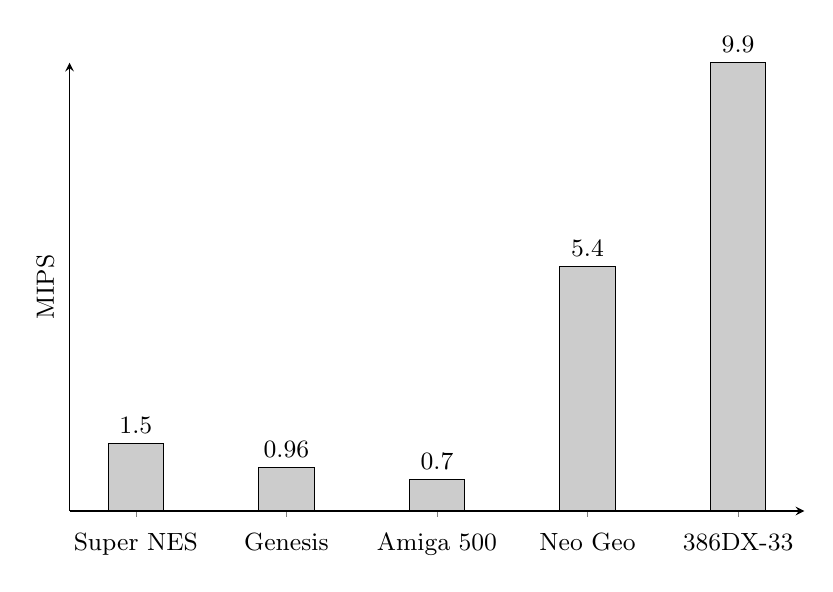
\begin{tikzpicture}[font=\small]
    \begin{axis}[
      width=0.9\textwidth,
      height=0.6\textwidth,
      ybar=6pt,
      bar width=20pt,
      ylabel={MIPS},
      ymin=0,
      ytick=\empty,
      xtick=data,
      axis x line=bottom,
      axis y line=left,
      enlarge x limits=0.11,
      symbolic x coords={Super NES,Genesis,Amiga 500,Neo Geo,386DX-33},
      xticklabel style={anchor=base,yshift=-\baselineskip},
      nodes near coords={\pgfmathprintnumber\pgfplotspointmeta}
    ]
      \addplot[fill=black!20,draw=black] coordinates {
        (Super NES,1.5)
        (Genesis,0.96)
        (Amiga 500,0.7)
        (Neo Geo,5.4)
        (386DX-33,9.9)
      };
    \end{axis}
   \end{tikzpicture}
   \caption{Game Console Vs PC: Raw power of the CPUs.} \label{fig:game_console_vs_PC}
 \end{figure}
 
PC had a fast CPU and a framebuffer but everything else was a nightmare:
\begin{itemize}
\item Smooth animation was next to impossible.
\item CPU could only do integer operations, 3D requires fractions.
\item RAM was segmented resulting in complex and error prone model.
\item The pixel of the VGA were not square: the framebuffer was distorted on screen.
\item Various sound systems had various capabilities and expectations.
\item Various RAM drivers exposed the RAM and made it available differently.
\end{itemize}

At first sight it did not look like much could be done to make a 3D game come true. Yet id made it happen thanks to creativity and hard work.

The book emphasis on the contrast between what the machine were theoritically capable of, the people who worked on it and the software they produced to innovate and reach new grounds:
\begin{itemize}
\item Chapter I: Hardware: The limits.
\item Chapter II: People: The team pushing the edges.
\item Chapter III: The result: Wolfenstein 3D engine.
\end{itemize}
Credited as the demise of all other types of computer such as the Amiga (reference HERE as footnote).\\
Ultimately all consoles abandonned the sprite engine and onboarded big fast cpus.\\
Racing the beam.\\
 \textbf{\underline{Disclaimer :}} The description that follows is technical and will most likely appeal to programmers. If you are more into the human aspect of game programming I would recommend instead to read David Kushner's chef d'oeuvre: "Masters of Doom".